\documentclass[11pt]{article}
\usepackage{homework}

\classname{322}
\homeworknum{4}



\begin{document}

% Environments

\newcommand{\state}[2]{\begin{statement}{#1} #2 \end{statement}}
\newcommand{\prob}[2]{\begin{problem}{#1} #2 \end{problem}}
\newcommand{\subprob}[1]{\begin{subproblem} #1 \end{subproblem}}
\newcommand{\sol}[1]{\begin{solution} #1 \end{solution}}
\newcommand{\fig}[2]{\begin{figure} \centering #2  \label{#1} \end{figure}}

\newcommand{\makebib}{
	\vfill
	\color{black}
	\nocite{*}
	\bibliography{references}{}
	\bibliographystyle{lucas_unsrt}
}
	

% Implication

\newcommand{\qwhere}{\quad \text{where} \quad}
\newcommand{\qimplies}{\quad \implies \quad}
\newcommand{\impliesq}{\implies \quad}



% Brackets

\newcommand{\paren}[1]{\left( #1 \right)}
\newcommand{\brac}[1]{\left[ #1 \right]}
\newcommand{\curly}[1]{\left\{ #1 \right\}}


% Greek

\newcommand{\alp}{\alpha}
\newcommand{\bet}{\beta}
\newcommand{\gam}{\gamma}
\newcommand{\del}{\delta}
\newcommand{\eps}{\epsilon}
\newcommand{\zet}{\zeta}
\newcommand{\tht}{\theta}
\newcommand{\kap}{\kappa}
\newcommand{\lam}{\lambda}
\newcommand{\sig}{\sigma}
\newcommand{\ups}{\upsilon}
\newcommand{\omg}{\omega}

\newcommand{\Gam}{\Gamma}
\newcommand{\Del}{\Delta}
\newcommand{\Tht}{\Theta}
\newcommand{\Lam}{\Lambda}
\newcommand{\Sig}{\Sigma}
\newcommand{\Omg}{\Omega}


% Text

\newcommand{\where}{\text{where }}

% Problem 1

\newcommand{\Hint}{H_\text{int}}
\newcommand{\ddcx}{\dd[3]{x}}
\newcommand{\psib}{\bar{\psi}}

\newcommand{\mh}{m_h}
\newcommand{\mmu}{m_\mu}
\newcommand{\me}{m_e}
\newcommand{\ma}{m_a}

\newcommand{\aexpt}{a_\text{expt.}}
\newcommand{\aQED}{a_\text{QED}}
\renewcommand{\GeV}{\giga\electronvolt}

\newcommand{\gamt}{\gam^5}



\state{(Jackson 14.1)}{
	Verify by explicit calculation that the {\Lienard}-Wiechert expressions for \emph{all} components of $\vE$ and $\vB$ for a particle moving with constant velocity agree with the ones obtained in the text by means of a Lorentz transformation.  Follow the general method at the end of Section~{14.1}.
}

\sol{
	The {\Lienard}-Wiechert expressions for the fields are given by Jackson~(14.13--14):
	\al{
		\vB &= [ \vn \cross \vE ]\ret, &
		\vE(\vx, t) &= e \brac{ \frac{\vn - \vbet}{\gam^2 (1 - \vbet \vdot \vn)^3 R^2} }\ret + \frac{e}{c} \brac{ \frac{\vn \cross \{ (\vn - \vbet) \cross \vbetd \}}{(1 - \vbet \vdot \vn)^3 R} }\ret.
	}
	For a particle moving with constant velocity, $\vbetd = 0$ and so $\vE(\vx, t)$ becomes
	\eq{
		\vE(\vx, t) = e \brac{ \frac{\vn - \vbet}{\gam^2 (1 - \vbet \vdot \vn)^3 R^2} }\ret.
	}
	
	The expressions for the components of $\vE$ and $\vB$ obtained by a Lorentz transformation are given by Jackson~(11.152):
	\al{
		\Eq &= -\frac{e \gam v t}{(b^2 + \gam^2 v^2 t^2)^{3/2}}, &
		\Ew &= \frac{e \gam b}{(b^2 + \gam^2 v^2 t^2)^{3/2}}, &
		\Ee &= \Bq = \Bw = 0, &
		\Be &= \bet \Ew,
	}
	where the particle is moving in the $\xq$ direction at impact parameter $b$, as shown in Fig.~\refeq{11.8}.  From Jackson~(14.16), note that
	\eq{
		[ (1 - \vbet \vdot \vn) R ]^2 = b^2 + v^2 t^2 - \bet^2 b^2
		= \frac{b^2 + \gam^2 v^2 t^2}{\gam}
	}
	
	\begin{figure}[b] \centering
		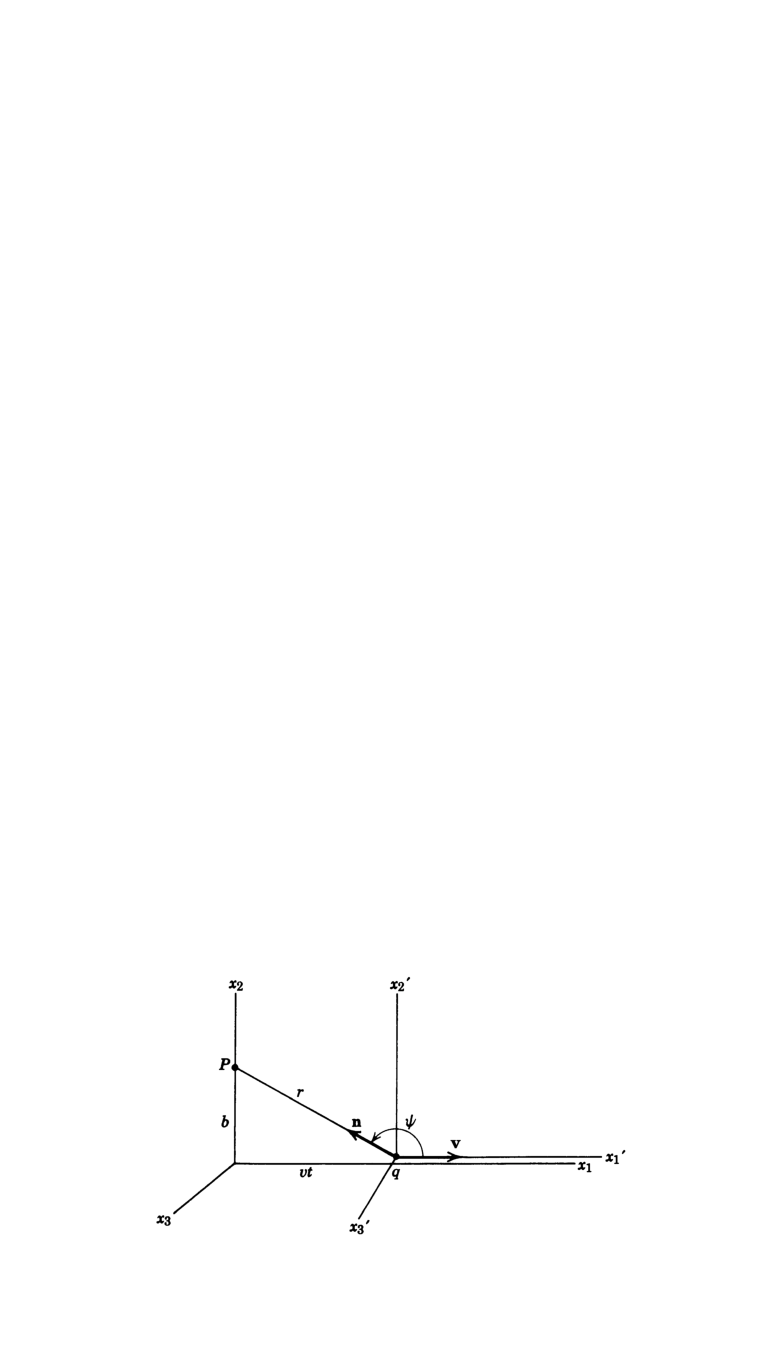
\includegraphics{11-8}
		\caption{(Jackson Fig.~11.8) Particle of charge $q$ moving at constant velocity $\vv$ passes an observation point $P$ at impact parameter $b$.}
		\label{11.8}
	\end{figure}

	
}



\clearpage
\state{(Jackson 14.3)}{
	The Heaviside-Feynman expression for the electric field of a particle of charge $e$ in arbitrary motion, an alternative to the {\Lienard}-Wiechert expression~(14.14) is
	\eq{
		\vE = e \brac{ \frac{\vn}{R^2} }\ret + e \brac{ \frac{R}{c} }\ret \dv{t} \brac{ \frac{\vn}{R^2} }\ret + \frac{e^2}{c^2} \dv[2]{t} [ \vn ]\ret,
	}
	where the time derivatives are with respect to the time at the observation point.  The magnetic fields are given by (14.3).
	
	Using the fact that the retarded time is $t' = t - R(t') / c$ and that, as a result,
	\eq{
		\dv{t}{t'} = 1 - \vbet(t') \vdot \vn(t'),
	}
	show that the form above yields (14.14) when the time differentiations are performed.
}



\state{(Jackson 14.4)}{
	Using the {\Lienard}-Wiechart fields, discuss the time-averaged power radiated per unit solid angle in nonrelativistic motion of a particle with charge $e$.  Sketch the angular distribution of the radiation and determine the total power radiated in each case.
}

\prob{}{
	The particle is moving along the $z$ axis with instantaneous position $z(t) = \alp \cos \omgo t$.
}

\prob{}{
	The particle is moving in a circle of radius $R$ in the $xy$ plane with constant angular frequency $\omgo$.
}


\makebib

\end{document}